\documentclass[journal]{IEEEtran}

\usepackage{cite}
\usepackage{amsmath,amssymb,amsfonts,amsthm,bm,mathtools}
\usepackage{graphicx}
\usepackage{booktabs,multirow,array}
\usepackage{float}
\usepackage{algorithm}
\usepackage{algpseudocode}
\usepackage{url}
\usepackage{color}
\usepackage{balance}
\usepackage[hidelinks]{hyperref}
\hypersetup{
  pdftitle={Energy-Efficient Hybrid STAR-RIS via Sparse Active Amplification and Gain Control},
  pdfauthor={Hongjian Huang, Yunpei Chen, Xingang Xie, Xiaonan Yang, Renjie Liang, Jinghui Qiu},
  pdfsubject={Hybrid active-passive STAR-RIS energy efficiency},
  pdfkeywords={STAR-RIS, active RIS, hybrid active-passive RIS, energy efficiency, spectral efficiency, Pareto boundary, amplifier noise}
}
\Urlmuskip=0mu plus 1mu\relax

\graphicspath{{./figs/}{../figs/}}

% Compact IEEE-style float and display spacing.
\setlength{\textfloatsep}{2pt plus 1pt minus 1pt}
\setlength{\floatsep}{2pt plus 1pt minus 1pt}
\setlength{\intextsep}{2pt plus 1pt minus 1pt}
\setlength{\abovedisplayskip}{3pt plus 1pt minus 1pt}
\setlength{\belowdisplayskip}{3pt plus 1pt minus 1pt}
\setlength{\abovedisplayshortskip}{2pt plus 1pt minus 1pt}
\setlength{\belowdisplayshortskip}{2pt plus 1pt minus 1pt}
\setlength{\jot}{1pt}

% Compact section/subsection spacing while preserving IEEEtran heading style.
\makeatletter
\def\section{\@startsection{section}{1}{\z@}{1.2ex plus 0.4ex minus 0.2ex}%
{0.35ex plus 0.2ex minus 0ex}{\normalfont\normalsize\centering\scshape}}%
\def\subsection{\@startsection{subsection}{2}{\z@}{1.05ex plus 0.35ex minus 0.2ex}%
{0.25ex plus 0.15ex minus 0ex}{\normalfont\normalsize\itshape}}%
\makeatother
\setlength{\abovecaptionskip}{1.5pt plus 0.5pt minus 0.5pt}
\setlength{\belowcaptionskip}{0pt}

\let\olditemize\itemize
\let\oldenditemize\enditemize
\renewenvironment{itemize}{\olditemize\setlength{\itemsep}{1pt}\setlength{\parskip}{0pt}\setlength{\parsep}{0pt}}{\oldenditemize}


\newtheorem{proposition}{Proposition}

\raggedbottom
\begin{document}

\title{Energy-Efficient Hybrid STAR-RIS via Sparse Active Amplification and Gain Control}

\author{Hongjian Huang, Yunpei Chen, Xingang Xie, Xiaonan Yang, Renjie Liang, and Jinghui Qiu%
\thanks{Corresponding author: Renjie Liang.}}
\maketitle


\begin{abstract}
Hybrid active-passive simultaneously transmitting and reflecting reconfigurable intelligent surfaces (STAR-RISs) can improve spectral efficiency (SE), yet their energy efficiency (EE) is constrained by amplifier noise and hardware power. This letter characterizes the EE-SE boundary through a multi-component power model covering BS transmit power, controller/bias power, switching overhead, and gain-dependent amplification power. An amplification on--off rule, a closed-form SE-oriented common-gain law, and a power-minimizing gain refinement are embedded into a finite-grid sparse-activation solver for ES, TS, and SS protocols. Simulations under Nakagami-$m$ fading show that sparse amplification improves moderate-to-high-SE operation by balancing BS-power reduction against active-noise and hardware overhead.
\end{abstract}

\begin{IEEEkeywords}
STAR-RIS, active RIS, hybrid active-passive RIS, energy efficiency, spectral efficiency, Pareto boundary, amplifier noise.
\end{IEEEkeywords}

\section{Introduction}
Reconfigurable intelligent surfaces (RISs) can enhance wireless propagation by passive beam manipulation \cite{wu2019irs}. STAR-RISs extend this capability to simultaneous transmission and reflection, enabling a common surface to serve users on both sides \cite{liu2021star,mu2022star}. This property is attractive for asymmetric two-side coverage, but purely passive STAR-RIS remains limited by multiplicative path loss.

Embedding sparse active elements can mitigate this loss, but the resulting gain is paid for through amplifier noise and hardware power \cite{ma2023activeee,peng2023hybrid,huang2024hybrid,zhang2022signal}. Measurement-driven studies further indicate that RIS power includes controller/bias and switching terms rather than a single constant \cite{wang2023static,wang2024practical}. In STAR-RIS, these effects are more pronounced because the two sides jointly compete for aperture, power split, and active hardware budget.


Existing active or hybrid STAR-RIS studies have addressed related scenarios, including NOMA and SWIPT \cite{yue2024astarsnoma,zhu2025activepassive}. Nevertheless, the joint effect of amplifier noise, sparse activation, dynamic switching overhead, and side-wise EE-SE tradeoff has not been characterized under a common boundary-generation framework. To address this gap, this letter makes four specific contributions. First, it formulates a multi-component STAR-RIS power model that separates BS PA power, controller/bias consumption, reconfiguration overhead, and gain-dependent amplification power. Second, it derives a side-wise gain structure that exposes when sparse amplification is SINR-beneficial and how the common gain should be refined for EE. Third, it embeds these rules into a finite-grid sparse solver with cost-aware ranking. Finally, it gives a unified ES/TS/SS boundary comparison and extracts design rules.

\section{System model}
\subsection{Hybrid active-passive STAR-RIS downlink}
Consider the downlink illustrated in Fig.~\ref{fig:system}, where a BS with $M$ antennas serves $K_t$ transmission-side users and $K_r$ reflection-side users through an $N$-element STAR-RIS. The user-index sets are $\mathcal{K}_t=\{1,\ldots,K_t\}$ and $\mathcal{K}_r=\{1,\ldots,K_r\}$. Under the ES protocol \cite{mu2022star}, the $n$th STAR-RIS element uses
\begin{equation}
\theta_{n,s}=\sqrt{\rho_{n,s}}\beta_{n,s}e^{j\phi_{n,s}},\qquad s\in\{t,r\},
\label{eq:theta}
\end{equation}
where $\rho_{n,s}$ is the power-splitting coefficient, $\beta_{n,s}$ is the amplification factor, and $\phi_{n,s}$ is the phase shift. The coefficients satisfy $\rho_{n,t}+\rho_{n,r}=1$, $0\le \rho_{n,s}\le 1$, and $1\le \beta_{n,s}\le \beta_{\max}$. Passive elements use $\beta_{n,s}=1$, while active elements use $\beta_{n,s}>1$ on their assigned side. Let $\mathcal{A}_t$ and $\mathcal{A}_r$ denote the active-element sets for transmission and reflection. Each active element is assigned to at most one side, so $\mathcal{A}_t\cap\mathcal{A}_r=\emptyset$, and $\mathcal{A}=\mathcal{A}_t\cup\mathcal{A}_r$.

\begin{figure}[!t]
\centering
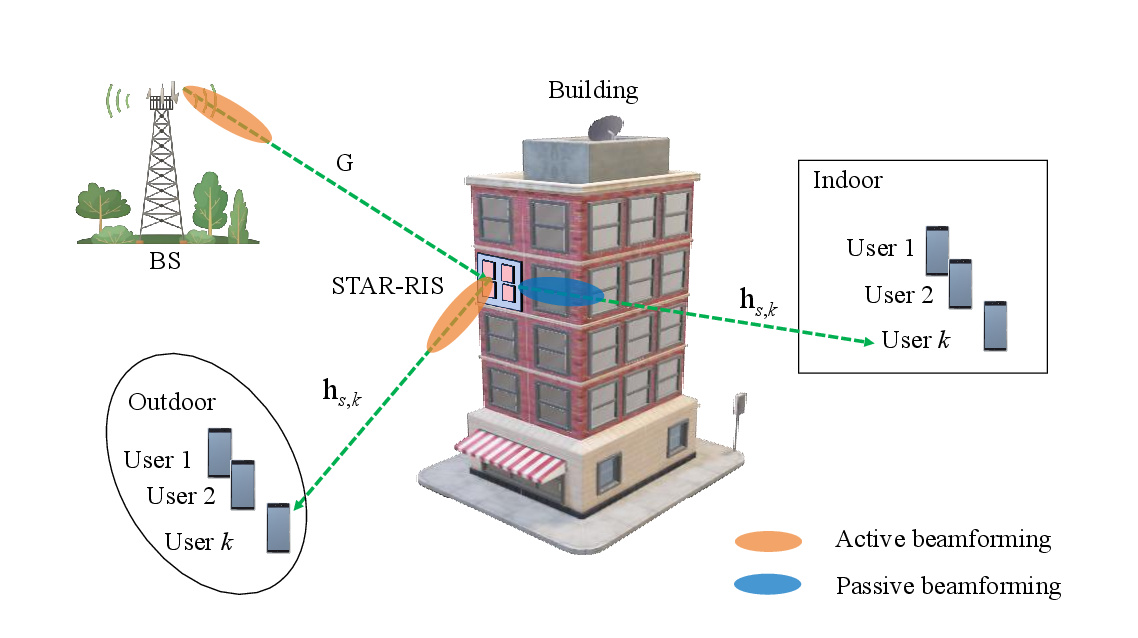
\includegraphics[width=0.90\columnwidth]{systemEE3_clean.jpg}
\caption{Hybrid active-passive STAR-RIS-assisted two-side downlink.}
\label{fig:system}
\end{figure}

Denote by $\mathbf{G}\in\mathbb{C}^{N\times M}$ the BS-to-STAR-RIS channel, and by $\mathbf{h}_{s,k}\in\mathbb{C}^N$ the STAR-RIS-to-user channel on side $s$ for user $k$. The received signal at user $(s,k)$ is
\begin{equation}
y_{s,k}=\mathbf{h}_{s,k}^H\mathbf{\Theta}_s\mathbf{G}
\sum_{s'\in\{t,r\}}\sum_{j\in\mathcal{K}_{s'}}\mathbf{w}_{s',j}x_{s',j}
+\mathbf{h}_{s,k}^H\mathbf{n}_{a,s}+n_{s,k},
\label{eq:received}
\end{equation}
where $\mathbf{\Theta}_s=\mathrm{diag}(\theta_{1,s},\ldots,\theta_{N,s})$, $\mathbf{w}_{s,j}\in\mathbb{C}^{M}$ is the BS beamformer for user $(s,j)$, $x_{s,j}$ is the unit-power information symbol, and $n_{s,k}\sim\mathcal{CN}(0,\sigma_0^2)$ is thermal noise. The vector $\mathbf{n}_{a,s}$ collects the amplified noise contributions from the active elements on side $s$. Following the active-RIS noise model in \cite{zhang2022signal,ma2023activeee}, the active-noise vector is modeled as
\begin{equation}
\mathbf{n}_{a,s}\sim\mathcal{CN}(\mathbf{0},\mathbf{C}_{a,s}),\qquad
\mathbf{C}_{a,s}=\mathrm{diag}(c_{1,s},\ldots,c_{N,s}),
\label{eq:na_stat}
\end{equation}
where $c_{n,s}=\rho_{n,s}\beta_{n,s}^2\sigma_a^2$ for $n\in\mathcal{A}_s$ and $c_{n,s}=0$ otherwise. Here, $\sigma_a^2$ is the input-referred active-element noise variance, and $\mathbf n_{a,s}$ denotes the equivalent amplified noise contribution. The SINR of user $(s,k)$ becomes
\begin{equation}
\gamma_{s,k}=
\frac{\left|\mathbf{h}_{s,k}^H\mathbf{\Theta}_s\mathbf{G}\mathbf{w}_{s,k}\right|^2}
{\sum_{\substack{s'\in\{t,r\},\ j\in\mathcal{K}_{s'}\\(s',j)\ne(s,k)}}
\left|\mathbf{h}_{s,k}^H\mathbf{\Theta}_s\mathbf{G}\mathbf{w}_{s',j}\right|^2
+\sigma_{a,s,k}^2+\sigma_0^2},
\label{eq:sinr_full}
\end{equation}
where $\sigma_{a,s,k}^2=\mathbf{h}_{s,k}^H\mathbf{C}_{a,s}\mathbf{h}_{s,k}$ is the active-noise term seen at user $(s,k)$.

\subsection{Power-consumption model}
Following measurement-based RIS power models \cite{wang2023static,wang2024practical}, the consumed power is
\begin{equation}
\begin{aligned}
P_{\mathrm{tot}}
&=\frac{1}{\eta_{\mathrm{PA}}}
\sum_{s\in\{t,r\}}\sum_{k\in\mathcal{K}_s}\|\mathbf{w}_{s,k}\|^2
+P_{\mathrm{ctrl}}+P_{\mathrm{bias}}|\mathcal{A}|  \\
&\quad +f_u\!\left(E_{\mathrm{sw},0}+E_{\mathrm{sw},1}|\mathcal{A}|\right) \\
&\quad +\sum_{n\in\mathcal{A}_t}\mu_t(\beta_{n,t}^2-1)
+\sum_{n\in\mathcal{A}_r}\mu_r(\beta_{n,r}^2-1),
\end{aligned}
\label{eq:power_model}
\end{equation}
where $\eta_{\mathrm{PA}}$ is the BS PA efficiency, $|\mathcal{A}|$ is the number of active elements, $P_{\mathrm{ctrl}}$ is the controller power, $P_{\mathrm{bias}}$ is the per-active-element bias power, $f_u$ is the update frequency, $E_{\mathrm{sw},0}$ and $E_{\mathrm{sw},1}$ are the base and per-active-element switching energies per update, and $\mu_t,\mu_r$ are gain-dependent amplifier-power coefficients. The four terms in \eqref{eq:power_model} represent the PA-normalized BS transmit power, static controller/bias power, update-rate-weighted switching power, and gain-dependent amplification power, respectively.

\subsection{Equivalent scalar model}
To obtain a tractable EE-SE boundary, the full model is reduced to an equivalent scalar form using four standard approximations: residual multiuser leakage in \eqref{eq:sinr_full} is neglected, common side-wise splitting and gain are used with $\rho_{n,s}=\rho_s$ and $\beta_{n,s}=\beta_s$ for $n\in\mathcal{A}_s$, dominant cascaded paths are phase-aligned, and the side target $R_s$ is enforced through equal per-user targets $R_s/K_s$.

Let $\mathbf v_{s,k}$ be a normalized post-ZF BS direction. The scalar BS-to-element gain is represented by the stream-averaged effective gain
\[
|g_n|\triangleq \frac{1}{K_t+K_r}\sum_{s\in\{t,r\}}\sum_{k\in\mathcal{K}_s}|[\mathbf{G}\mathbf v_{s,k}]_n|.
\]
With $h_{s,k,n}$ denoting the $n$th entry of $\mathbf{h}_{s,k}$, define
\begin{equation}
u_{s,k,n} = |g_n|\,|h_{s,k,n}|.
\label{eq:un}
\end{equation}
Then the side-wise effective coherent term for user $(s,k)$ is
\begin{equation}
\psi_{s,k}(\beta_s)=
\sum_{n\in\mathcal{P}_s}\sqrt{\rho_s}u_{s,k,n}
+\beta_s\sum_{n\in\mathcal{A}_s}\sqrt{\rho_s}u_{s,k,n},
\label{eq:psi}
\end{equation}
where $\mathcal{P}_s=\{1,\ldots,N\}\setminus\mathcal{A}_s$ contains passive elements and those active only for the opposite side. The corresponding active-noise term is
\begin{equation}
\zeta_{s,k}(\beta_s)=\sigma_0^2+
\rho_s\beta_s^2\sigma_a^2
\sum_{n\in\mathcal{A}_s}|h_{s,k,n}|^2.
\label{eq:noise_exact}
\end{equation}
Under the equal per-user target $R_s/K_s$, the minimum side power for meeting side target $R_s$ is
\begin{equation}
p_s^{\min}(\beta_s)=
\sum_{k\in\mathcal{K}_s}
\frac{(2^{R_s/K_s}-1)\zeta_{s,k}(\beta_s)}{\psi_{s,k}^2(\beta_s)}.
\label{eq:minsidepower}
\end{equation}

\section{Problem formulation}
The sum spectral efficiency and normalized energy efficiency are
\begin{align}
R_\Sigma
&= \sum_{s\in\{t,r\}}\sum_{k\in\mathcal{K}_s}\log_2(1+\gamma_{s,k}),
\label{eq:sumrate}\\
\mathrm{EE}_{\mathrm{norm}}
&= \frac{R_\Sigma}{P_{\mathrm{tot}}}\quad \text{(bit/J/Hz)}.
\label{eq:ee}
\end{align}
For bandwidth $B$, the physical EE equals $BR_\Sigma/P_{\mathrm{tot}}$ in bit/J. The normalized metric in \eqref{eq:ee} is used throughout. Let $\mathcal X\triangleq\{\mathbf W,\rho_t,\rho_r,\bm\phi,\beta_t,\beta_r,\mathcal A_t,\mathcal A_r\}$. The corresponding normalized-EE maximization problem is
\begin{equation}
\begin{aligned}
\max_{\mathcal X}
\quad & \frac{R_\Sigma}{P_{\mathrm{tot}}} \\
\text{s.t.}\quad &
\log_2(1+\gamma_{s,k})\ge \bar{R}_{s,k},\ \forall s,k, \\
&
\sum_{s\in\{t,r\}}\sum_{k\in\mathcal{K}_s}\|\mathbf{w}_{s,k}\|^2 \le P_{\max}^{\mathrm{BS}},\\
&
1\le \beta_s\le \beta_{\max},\quad s\in\{t,r\},\\
&
\mathcal{A}_t\cap\mathcal{A}_r=\emptyset,\quad \mathcal{A}=\mathcal{A}_t\cup\mathcal{A}_r,\\
&
\rho_t+\rho_r=1,\quad 0\le \rho_s\le 1,\quad s\in\{t,r\},\\
&
\rho_s\beta_s^2\sigma_a^2 \le \Gamma_s,\quad s\in\{t,r\}.
\end{aligned}
\label{eq:P0}
\end{equation}
Here, $\Gamma_s$ is an optional side-wise noise-injection or hardware-safety limit. Problem \eqref{eq:P0} is non-convex because its fractional objective couples beamforming, STAR coefficients, common gains, and active-set selection.

To trace an EE-SE Pareto-boundary approximation, the $\epsilon$-constraint formulation is adopted
\begin{equation}
\begin{aligned}
\mathcal{P}(\epsilon):\quad
\min_{\mathcal X}
\quad & P_{\mathrm{tot}} \\
\text{s.t.}\quad &
R_\Sigma \ge \epsilon, \\
& \text{constraints of \eqref{eq:P0}.}
\end{aligned}
\label{eq:epsilon}
\end{equation}
In the solver, the generic QoS terms are instantiated as $\bar R_{s,k}=R_s/K_s$ with $R_t=\alpha\epsilon$ and $R_r=(1-\alpha)\epsilon$, so the per-user constraints realize the side targets in \eqref{eq:minsidepower}. Since the solver uses structured sparse activation and finite grids, the generated curve is an achievable Pareto-boundary approximation rather than a certified global optimum. The model structure is then exploited to derive transferable design rules.

\section{Gain structure}
\subsection{Amplification on--off criterion}
Given a side support, the key decision is whether the common active gain should be switched on, i.e., whether increasing $\beta_s$ above one improves the side-wise SINR. Define
\begin{equation}
\begin{aligned}
a_s &= \min_k \sum_{n\in\mathcal{P}_s}\sqrt{\rho_s}u_{s,k,n},\\
b_s &= \min_k \sum_{n\in\mathcal{A}_s}\sqrt{\rho_s}u_{s,k,n},\\
c_s &= \sigma_0^2,\\
d_s &= \max_k \rho_s\sigma_a^2\sum_{n\in\mathcal{A}_s}|h_{s,k,n}|^2 .
\end{aligned}
\label{eq:abcd}
\end{equation}
Here, $a_s$ and $b_s$ are conservative worst-user coherent-gain aggregates from passive and active contributions, while $c_s$ and $d_s$ are the thermal-noise baseline and active-noise coefficient. Let $\bar p_s$ denote an auxiliary normalized side power used only for this local monotonicity analysis. The worst-user SINR lower bound is
\begin{equation}
\underline{\gamma}_s(\beta_s)=
\frac{\bar{p}_s(a_s+b_s\beta_s)^2}{c_s+d_s\beta_s^2}.
\label{eq:surrogate}
\end{equation}
The coherent term grows linearly with $\beta_s$, whereas the injected active noise grows quadratically. Differentiating \eqref{eq:surrogate} gives
\begin{equation}
\frac{\mathrm{d}\underline{\gamma}_s}{\mathrm{d}\beta_s}=
\frac{2\bar{p}_s(a_s+b_s\beta_s)(b_sc_s-a_sd_s\beta_s)}{(c_s+d_s\beta_s^2)^2}.
\label{eq:surrogate_derivative}
\end{equation}
Thus, at the passive-gain point $\beta_s=1$, amplification is locally useful if
\begin{equation}
\left.\frac{\mathrm{d}\underline{\gamma}_s}{\mathrm{d}\beta_s}\right|_{\beta_s=1}>0
\iff b_sc_s>a_sd_s.
\label{eq:threshold}
\end{equation}
Equation \eqref{eq:threshold} gives the amplification on--off criterion: the active coherent-gain aggregate $b_s$, weighted by the thermal-noise baseline $c_s$, must dominate the passive coherent-gain aggregate $a_s$ weighted by the active-noise coefficient $d_s$. When this inequality holds, amplification is locally beneficial for the SINR lower bound. Otherwise, the amplifier should remain off in this local test. Bias, switching, and amplification-power costs further tighten the final activation decision.

\begin{proposition}\label{prop:se_optimal}
For the regular hybrid active-passive case $a_s>0$, $b_s>0$, $c_s>0$, and $d_s>0$, $\underline{\gamma}_s(\beta_s)$ is unimodal on $[1,\beta_{\max}]$. Its SE-oriented gain is
\begin{equation}
\beta_{s,\mathrm{SE}}^\star=
\left[\frac{b_sc_s}{a_sd_s}\right]_{[1,\beta_{\max}]},
\label{eq:beta_closed}
\end{equation}
where $[x]_{[l,u]}=\min\{u,\max\{l,x\}\}$. The non-regular cases follow from the same derivative behavior. If $b_s=0$, set $\beta_{s,\mathrm{SE}}^\star=1$. If $a_s=0$ with $b_s>0$, or if $d_s=0$ with $b_s>0$, $\underline{\gamma}_s(\beta_s)$ is nondecreasing and $\beta_{s,\mathrm{SE}}^\star=\beta_{\max}$. If $|\mathcal{A}_s|=0$, set $\beta_s=1$.
\end{proposition}

\begin{IEEEproof}
In the regular case, the sign of \eqref{eq:surrogate_derivative} is determined only by $b_sc_s-a_sd_s\beta_s$, which changes sign once. Hence \eqref{eq:surrogate} is unimodal and the stationary point is $b_sc_s/(a_sd_s)$, clipped to $[1,\beta_{\max}]$. The boundary cases follow directly from \eqref{eq:surrogate_derivative}: $b_s=0$ makes the derivative non-positive, while $a_s=0$ with $b_s>0$ or $d_s=0$ with $b_s>0$ makes \eqref{eq:surrogate} nondecreasing.
\end{IEEEproof}

\subsection{Power-minimizing gain}
The gain in \eqref{eq:beta_closed} is SE-oriented. EE optimization must also account for BS transmit power and active-amplifier power. For a target side rate $R_s$, define the side-wise cost $\Psi_s(\beta_s)$ as the sum of the transmit-power term induced by \eqref{eq:minsidepower} under the worst-user coefficients and the gain-dependent active-amplifier power:
\begin{align}
\Psi_s(\beta_s)
&=\frac{K_s(2^{R_s/K_s}-1)(c_s+d_s\beta_s^2)}{\eta_{\mathrm{PA}}(a_s+b_s\beta_s)^2}
+\mu_s|\mathcal{A}_s|(\beta_s^2-1),
\label{eq:side_cost}\\
\Psi_s'(\beta_s)
&=\frac{2K_s(2^{R_s/K_s}-1)(a_sd_s\beta_s-b_sc_s)}{\eta_{\mathrm{PA}}(a_s+b_s\beta_s)^3}
+2\mu_s|\mathcal{A}_s|\beta_s,
\label{eq:side_derivative}\\
\Psi_s''(\beta_s)
&=\frac{2K_s(2^{R_s/K_s}-1)}{\eta_{\mathrm{PA}}(a_s+b_s\beta_s)^4}
\Big(a_s^2d_s-2a_sb_sd_s\beta_s+3b_s^2c_s\Big) \notag\\
&\quad +2\mu_s|\mathcal{A}_s|.
\label{eq:side_second}
\end{align}

\begin{proposition}\label{prop:convexity}
Assume the hybrid active-passive case $a_s>0$, $b_s>0$, and $d_s>0$. Under the condition
\begin{equation}
\beta_{\max}
\le
\frac{a_s^2d_s+3b_s^2c_s}{2a_sb_sd_s},
\label{eq:convexity_cond}
\end{equation}
$\Psi_s(\beta_s)$ is strictly convex on $[1,\beta_{\max}]$. Consequently, the side-wise power-minimizing gain is unique and is obtained by checking the two endpoints and the interior stationary point solving \eqref{eq:side_derivative}, if it lies in $[1,\beta_{\max}]$.
\end{proposition}

\begin{IEEEproof}
Under \eqref{eq:convexity_cond}, the bracketed term in \eqref{eq:side_second} is non-negative on $[1,\beta_{\max}]$. Since $|\mathcal{A}_s|>0$ and $\mu_s>0$, the term $2\mu_s|\mathcal{A}_s|$ yields $\Psi_s''(\beta_s)>0$ over the interval. Hence $\Psi_s$ is strictly convex and has a unique minimizer.
\end{IEEEproof}


Condition \eqref{eq:convexity_cond} is sufficient but not necessary. When it is violated, $\Psi_s(\beta_s)$ remains continuous on $[1,\beta_{\max}]$, so a bounded one-dimensional search is still well-defined. In the simulations, $\beta_s=1$ is used for fully passive or zero-active-coherent cases. Otherwise, $\Psi_s(\beta_s)$ is minimized over $[1,\beta_{\max}]$, with \eqref{eq:beta_closed} used only as an SE-oriented reference or initialization.

\subsection{Extension to TS and SS}
Since ES is covered by \eqref{eq:abcd}, for $p\in\{\mathrm{TS},\mathrm{SS}\}$ let $\mathcal{P}_s^{(p)}$ and $\mathcal{A}_s^{(p)}$ denote the passive and active support sets. Define
\begin{align*}
a_s^{(p)} &= \min_k \sum_{n\in\mathcal{P}_s^{(p)}} u_{s,k,n},\\
b_s^{(p)} &= \min_k \sum_{n\in\mathcal{A}_s^{(p)}} u_{s,k,n},\\
c_s^{(p)} &= \sigma_0^2,\\
d_s^{(p)} &= \max_k \sigma_a^2 \sum_{n\in\mathcal{A}_s^{(p)}} |h_{s,k,n}|^2.
\end{align*}
For TS, $\mathcal{P}_s^{(\mathrm{TS})}=\{1,\ldots,N\}\setminus\mathcal{A}_s$ and the effective target becomes $R_s/\tau_s$. Its consumed power is time-averaged:
\begin{equation}
\begin{aligned}
P_{\mathrm{tot}}^{\mathrm{TS}}
&=P_{\mathrm{ctrl}}+P_{\mathrm{bias}}|\mathcal{A}|
+f_u\!\left(E_{\mathrm{sw},0}+E_{\mathrm{sw},1}|\mathcal{A}|\right) \\
&\quad +\sum_{s\in\{t,r\}}\tau_s\!\left(\frac{P_{\mathrm{tx},s}}{\eta_{\mathrm{PA}}}
+\mu_s|\mathcal{A}_s|(\beta_s^2-1)\right),
\end{aligned}
\label{eq:ts_power}
\end{equation}
where $P_{\mathrm{tx},s}$ is the BS transmit power in slot $s$. For SS, $\mathcal{P}_s^{(\mathrm{SS})}=\mathcal{S}_s\setminus\mathcal{A}_s$, with $\mathcal{S}_t\cup\mathcal{S}_r=\{1,\ldots,N\}$ and $\mathcal{S}_t\cap\mathcal{S}_r=\emptyset$. The ES rules then apply after replacing $(a_s,b_s,c_s,d_s)$ by $(a_s^{(p)},b_s^{(p)},c_s^{(p)},d_s^{(p)})$ and using the corresponding consumed-power denominator.


\section{Sparse activation algorithm}
For a target sum-SE level $\epsilon$, Algorithm~\ref{alg:solver} scans the $L$- and $\alpha$-grids, forms a compact pool of side-specific active supports, updates $\beta_s$, and retains the feasible candidate $(\mathcal{A}_t,\mathcal{A}_r,\beta_t,\beta_r,\alpha)$ with the minimum consumed power.

\subsection{Grid search over sparsity and rate split}
The outer grid contains the active-cardinality budget $L\in\mathcal{L}$ and the side-rate split $\alpha\in\mathcal{G}_{\alpha}$. For each pair $(L,\alpha)$, the side targets are
\[
R_t=\alpha\epsilon,\qquad R_r=(1-\alpha)\epsilon.
\]
Thus, $L$ controls hardware sparsity, while $\alpha$ controls traffic asymmetry. Each grid point defines one candidate design subproblem: select $L$ active elements, assign them to sides, update $(\beta_t,\beta_r)$, evaluate the constraints of \eqref{eq:P0}, and compare the resulting $P_{\mathrm{tot}}$.

\subsection{Active-set construction}
For a fixed $(L,\alpha)$, candidate supports are constructed by testing whether an inactive element $n\notin\mathcal{A}_s$ should be switched on for side $s$. The test uses the first-order change of the side-wise cost in \eqref{eq:side_cost}. Define
\[
C_s=\frac{K_s(2^{R_s/K_s}-1)}{\eta_{\mathrm{PA}}},
\]
which collects the side-rate and PA-efficiency factors in the transmit-power term. Introduce a relaxed activation variable $x_{n,s}\in[0,1]$, with $x_{n,s}=0$ denoting inactive and $x_{n,s}=1$ denoting active. Switching on element $n$ changes its coefficient from passive gain $1$ to active gain $\beta_s$, giving the worst-user coherent increment
\[
\Delta u_{n,s}=\sqrt{\rho_s}|g_n|\min_k|h_{s,k,n}|.
\]
The coherent denominator is therefore perturbed as
\[
D_{n,s}(x_{n,s})=a_s+b_s\beta_s+(\beta_s-1)x_{n,s}\Delta u_{n,s}.
\]
The active-noise coefficient changes from $d_s$ to $d_s+x_{n,s}\Delta d_{n,s}$. The increment involves the post-insertion maximizing user and is nonsmooth. For ranking and first-order differentiation, the following approximation is used:
\[
\Delta d_{n,s}\approx \rho_s\sigma_a^2\overline{|h_{s,k,n}|^2},
\]
where
\[
\overline{|h_{s,k,n}|^2}\triangleq \frac{1}{K_s}\sum_{k\in\mathcal{K}_s}|h_{s,k,n}|^2.
\]
Substituting these perturbations into the cost in \eqref{eq:side_cost} gives
\[
\begin{aligned}
\Psi_s(x_{n,s})
&\approx
C_s\frac{c_s+\beta_s^2(d_s+x_{n,s}\Delta d_{n,s})}{D_{n,s}^2(x_{n,s})} \\
&\quad +\mu_s(|\mathcal{A}_s|+x_{n,s})(\beta_s^2-1)\\
&\quad +x_{n,s}(P_{\mathrm{bias}}+f_uE_{\mathrm{sw},1}).
\end{aligned}
\]
Differentiating at $x_{n,s}=0$ gives
\[
\begin{aligned}
\left.\frac{\partial \Psi_s}{\partial x_{n,s}}\right|_{x_{n,s}=0}
&= -\kappa_{1,s}\Delta u_{n,s}+\kappa_{2,s}\Delta d_{n,s} \\
&\quad +P_{\mathrm{bias}}+f_uE_{\mathrm{sw},1}
+\mu_s(\beta_s^2-1),
\end{aligned}
\]
where
\[
\kappa_{1,s}=\frac{2C_s(c_s+d_s\beta_s^2)(\beta_s-1)}{(a_s+b_s\beta_s)^3},
\qquad
\kappa_{2,s}=\frac{C_s\beta_s^2}{(a_s+b_s\beta_s)^2}.
\]
Hence, element $n$ is beneficial in the first-order sense when
\[
\tilde{\xi}_{n,s}\triangleq
\frac{\kappa_{1,s}\Delta u_{n,s}}
{\kappa_{2,s}\Delta d_{n,s}+P_{\mathrm{bias}}+f_uE_{\mathrm{sw},1}+\mu_s(\beta_s^2-1)} > 1.
\]
This condition indicates that the transmit-power saving from coherent-gain improvement must exceed the active-noise, bias/switching, and amplifier-power penalties.

For low-complexity ranking, the normalized scores are
\begin{equation}
\begin{aligned}
\xi_{n,t}
&=\frac{\alpha\sqrt{\rho_t}|g_n|\min_k|h_{t,k,n}|}
{\lambda_1\rho_t\sigma_a^2\overline{|h_{t,k,n}|^2}
+\lambda_2(P_{\mathrm{bias}}+f_uE_{\mathrm{sw},1})},\\
\xi_{n,r}
&=\frac{(1-\alpha)\sqrt{\rho_r}|g_n|\min_k|h_{r,k,n}|}
{\lambda_1\rho_r\sigma_a^2\overline{|h_{r,k,n}|^2}
+\lambda_2(P_{\mathrm{bias}}+f_uE_{\mathrm{sw},1})},
\end{aligned}
\label{eq:score}
\end{equation}
where $\lambda_1=\sigma_0^{-2}$ and $\lambda_2=(P_{\max}^{\mathrm{BS}})^{-1}$ are normalization weights. The scores in \eqref{eq:score} generate candidate supports: for each element, the larger side-wise score determines its assigned side, and the top $L$ elements form one candidate support. A strength-only ranker using the corresponding channel-only numerators in \eqref{eq:score} forms a second support and is reported as the ``strongest greedy'' baseline. After gain update, all candidates are re-evaluated using \eqref{eq:power_model}, \eqref{eq:minsidepower}, and \eqref{eq:side_cost}.

\subsection{Gain update}
For each candidate $(\mathcal{A}_t,\mathcal{A}_r)$, the solver computes $(a_s,b_s,c_s,d_s)$ for $s\in\{t,r\}$ and updates $\beta_s$ on each side. If $|\mathcal{A}_s|=0$ or $b_s=0$, no useful active coherent term is available and $\beta_s=1$ is set. Otherwise, the gain update solves
\[
\min_{\beta_s\in[1,\beta_{\max}]}\Psi_s(\beta_s).
\]
The updated gains determine the BS power through \eqref{eq:minsidepower}. The candidate is feasible if it satisfies the BS power budget, the bound $1\le\beta_s\le\beta_{\max}$, non-overlapping active supports $(\mathcal{A}_t\cap\mathcal{A}_r=\emptyset)$, protocol-specific ES/TS/SS constraints, and the optional safety limit $\Gamma_s$, i.e., the constraints of \eqref{eq:P0} under the scalar model. Among all feasible candidates for the current $\epsilon$, the one with the smallest $P_{\mathrm{tot}}$ is retained as the boundary point.

\begin{algorithm}[H]
\caption{Sparse-Activation Solver}
\label{alg:solver}
\begin{algorithmic}[1]
\Require Target $\epsilon$, grids $\mathcal{L}$, $\mathcal{G}_\alpha$, maximum gain $\beta_{\max}$
\Ensure Minimum-power feasible candidate
\State Initialize $P_{\min}\gets+\infty$ and best $\gets\emptyset$.
\ForAll{$(L,\alpha)\in\mathcal{L}\times\mathcal{G}_\alpha$}
    \State Build two ranked supports.
    \State Update $(\beta_t,\beta_r)$, evaluate BS power and $P_{\mathrm{tot}}$.
    \State Retain any feasible lower-power candidate.
\EndFor
\State \Return best.
\end{algorithmic}
\end{algorithm}

\subsection{Complexity}
Let $G=|\mathcal{G}_{\alpha}|$, $L_g=|\mathcal{L}|$, $K=K_t+K_r$, and $Q_\beta$ denote the bounded one-dimensional gain-search budget. For each boundary point, score computation, sorting, support evaluation, and gain update require $\mathcal{O}(L_gG(N\log N+NK+Q_{\beta}))$ operations. For $E$ sampled SE targets, the total complexity is $\mathcal{O}(E L_gG(N\log N+NK+Q_{\beta}))$, with memory dominated by channel coefficients and element scores.


\section{Numerical results}
All numerical settings are listed in Table~\ref{tab:params}. All plotted Monte-Carlo (MC) points average 10000 independent channel realizations with seeds $1$--$10000$. For reproducibility, the source code is available at \url{https://github.com/hjhuang1989-svg/hybrid-star-ris}.

\begin{table}[H]
\caption{Simulation parameters}
\label{tab:params}
\centering
\scriptsize
\setlength{\tabcolsep}{2pt}
\renewcommand{\arraystretch}{0.95}
\begin{tabular}{@{}>{\raggedright\arraybackslash}p{0.59\linewidth}>{\raggedright\arraybackslash}p{0.35\linewidth}@{}}
\toprule
\textbf{Parameter} & \textbf{Value} \\
\midrule
Elems./users $(N/K_t/K_r)$ & $24$ / $2$ / $2$ \\
Nakagami $(m_{BR}/m_{RU})$ & $1.0$ / $1.0$ \\
Avg. powers $(\Omega_{BR}/\Omega_t/\Omega_r)$ & $0.20$ / $(0.060,0.050)$ / $(0.080,0.060)$ \\
ES/TS split $(\rho_t,\rho_r)/(\tau_t,\tau_r)$ & $(0.55,0.45)$ / $(0.55,0.45)$ \\
Noise std. $(\sigma_0/\sigma_a)$ & $0.25$ / $0.05$ \\
Caps $(\beta_{\max}/P_{\max}^{\mathrm{BS}}\,[\mathrm{W}])$ & $5$ / $5.0$ \\
Ctrl./bias $(P_{\mathrm{ctrl}}/P_{\mathrm{bias}}\,[\mathrm{W}])$ & $0.10$ / $0.015$ \\
Switching $(f_u/E_{\mathrm{sw},0}/E_{\mathrm{sw},1})$ & $50$ Hz / $2.0\!\times\!10^{-4}$ J / $1.2\!\times\!10^{-4}$ J \\
Amp./PA $(\mu_t/\mu_r\,[\mathrm{W}]/\eta_{\mathrm{PA}})$ & $0.0025$ / $0.0025$ / $0.40$ \\
Grids $(\mathcal{G}_{\alpha}/\mathcal{L})$ & $\{0.20,0.25,\ldots,0.80\}$ / $\{0,3,\ldots,24\}$ \\
Fixed-unif./rand $(L/Q_{\mathrm{rand}})$ & $6$ / $1$ \\
Safety cap $(\Gamma_s)$ & inactive \\
\bottomrule
\end{tabular}
\end{table}

For ES, the baselines are passive ($L=0$), fixed uniform ($L=6$ linearly spaced indices $\{1,5,10,14,19,24\}$), optimized uniform (linearly spaced support with $L\in\mathcal L$), single-random sparse (one random support per $(L,\alpha)$, assigned by the larger score), strongest greedy (same grid with channel-strength ranking only), and active ($L=N$). A stronger $Q_{\mathrm{rand}}=20$ random-search audit is stored in the reproducibility results and does not change the main ordering at $R_\Sigma=12$.

Fig.~\ref{fig:pareto} shows the ES EE-SE boundary and the core power-allocation tradeoff. Passive STAR-RIS is competitive at low SE, but its BS-power requirement grows rapidly with $R_\Sigma$ and becomes infeasible once it exceeds $P_{\max}^{\mathrm{BS}}$. The unfilled passive markers at $R_\Sigma=18$ and $20$ bit/s/Hz are averaged over feasible trials only, with $p_f=0.98$ and $0.72$. The active benchmark lowers BS power but pays large static, switching, and amplification overhead. Compared with strongest greedy, the proposed ranker penalizes active-noise and hardware costs, preserving most coherent gain with lower consumed power. At $R_\Sigma=12$ bit/s/Hz, the proposed EE is $8.94$ bit/J/Hz, improving over fixed uniform, optimized uniform, single-random sparse, active, and passive by $33.1\%$, $19.4\%$, $15.2\%$, $32.4\%$, and $94.8\%$, respectively.

\begin{figure}[H]
\centering

\includegraphics[width=0.80\columnwidth]{fig_pareto_boundary.jpg}
\caption{Approximated ES EE-SE boundary. Unfilled passive markers denote rate points where not all trials are feasible. The label $p_f$ gives the feasible-trial fraction.}
\label{fig:pareto}
\end{figure}

Fig.~\ref{fig:design} compares ES, TS, and SS in terms of active ratio and common gain. The gains increase with target SE and approach $\beta_{\max}$ when rate pressure dominates. TS requires the densest active set because slot targets inflate by $1/\tau_s$, whereas ES and SS maintain lower active ratios with comparable gains. At $R_\Sigma=12$ bit/s/Hz, the ES/TS/SS active ratios are about $0.29/0.53/0.31$, with average gains $4.70/4.96/4.64$.

\begin{figure}[H]
\centering
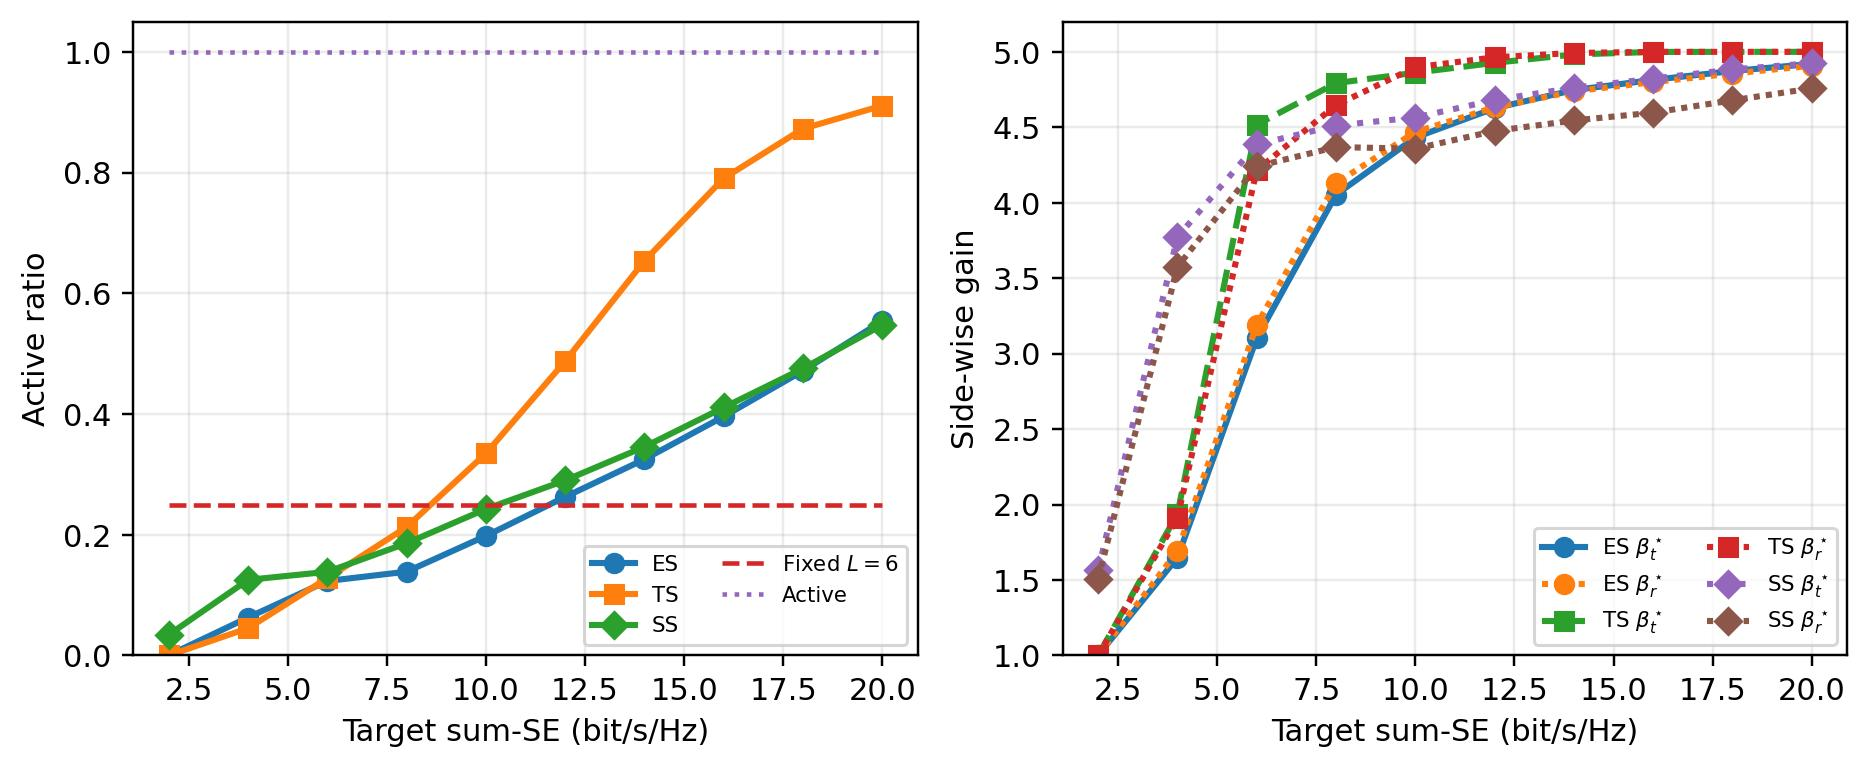
\includegraphics[width=0.90\columnwidth]{fig_design_rules.jpg}
\caption{Cross-mode ES/TS/SS design rules: active ratio and side-wise common gain.}
\label{fig:design}
\end{figure}

Fig.~\ref{fig:noise_dyn} shows ES hardware sensitivity at $R_\Sigma=6$, $9$, $12$, $15$, and $18$ bit/s/Hz. A larger gain is not always beneficial: increasing $\sigma_a$ suppresses the selected gain because amplifier noise scales with $\beta_s^2$ and raises the required power. A larger $f_u$ likewise increases switching power and reduces EE.

\begin{figure}[H]
\centering

\includegraphics[width=0.90\columnwidth]{fig_noise_dynamic.jpg}
\caption{ES hardware sensitivity versus amplifier noise and switching overhead.}
\label{fig:noise_dyn}
\end{figure}

Fig.~\ref{fig:breakdown} compares ES power at $R_\Sigma=12$ and $16$ bit/s/Hz. At $R_\Sigma=12$, active operation minimizes BS power ($0.67$ W) but incurs large overhead, whereas passive operation needs $2.64$ W. The proposed sparse design achieves the lowest total power, about $1.37$ W, and the same trend persists at $R_\Sigma=16$.

\begin{figure}[H]
\centering

\includegraphics[width=0.90\columnwidth]{fig_power_breakdown.jpg}
\caption{ES power breakdown at $R_\Sigma=12$ and $16$ bit/s/Hz.}
\label{fig:breakdown}
\end{figure}

\section{Conclusion}
This letter characterized the EE-SE tradeoff of hybrid active-passive STAR-RIS with sparse active amplification and gain control. An amplification on--off criterion, an SE-oriented gain law, and a power-minimizing gain refinement were embedded into a finite-grid sparse-activation solver. Numerical results show that sparse hybrid activation avoids both passive BS-power burden and full-array active overhead. Future work will validate the design under full-dimensional beamforming and incorporate signal-dependent active-output constraints.

\begingroup
\renewcommand{\baselinestretch}{0.70}\selectfont
\fontsize{5.2}{5.2}\selectfont
\begin{thebibliography}{99}
\setlength{\itemsep}{0pt}
\setlength{\parskip}{0pt}


\bibitem{wu2019irs}
Q.~Wu and R.~Zhang,
``Intelligent reflecting surface enhanced wireless network via joint active and passive beamforming,''
\emph{IEEE Trans. Wireless Commun.}, vol.~18, no.~11, pp.~5394--5409, Nov.~2019.


\bibitem{liu2021star}
Y.~Liu, X.~Mu, J.~Xu, R.~Schober, Y.~Hao, H.~V. Poor, and L.~Hanzo,
``STAR: Simultaneous transmission and reflection for 360$^\circ$ coverage by intelligent surfaces,''
\emph{IEEE Wireless Commun.}, vol.~28, no.~6, pp.~102--109, Dec.~2021.

\bibitem{mu2022star}
X.~Mu, Y.~Liu, L.~Guo, J.~Lin, and R.~Schober,
``Simultaneously transmitting and reflecting (STAR) RIS aided wireless communications,''
\emph{IEEE Trans. Wireless Commun.}, vol.~21, no.~5, pp.~3083--3098, May~2022.

\bibitem{ma2023activeee}
Y.~Ma, M.~Li, Y.~Liu, Q.~Wu, and Q.~Liu,
``Active reconfigurable intelligent surface for energy efficiency in MU-MISO systems,''
\emph{IEEE Trans. Veh. Technol.}, vol.~72, no.~3, pp.~4103--4107, Mar.~2023.

\bibitem{peng2023hybrid}
Q.~Peng, Q.~Wu, G.~Chen, R.~Liu, S.~Ma, and W.~Chen,
``Hybrid active-passive IRS assisted energy-efficient wireless communication,''
\emph{IEEE Commun. Lett.}, vol.~27, no.~8, pp.~2202--2206, Aug.~2023.

\bibitem{huang2024hybrid}
A.~Huang, X.~Mu, L.~Guo, and G.~Zhu,
``Hybrid active-passive RIS transmitter enabled energy-efficient multi-user communications,''
\emph{IEEE Trans. Wireless Commun.}, vol.~23, no.~9, pp.~10653--10666, Sep.~2024.

\bibitem{zhang2022signal}
Z.~Zhang, L.~Dai, X.~Chen, C.~Liu, F.~Yang, R.~Schober, and H.~V. Poor,
``Active RISs: Signal modeling, asymptotic analysis, and beamforming design,''
in \emph{Proc. IEEE GLOBECOM}, Rio de Janeiro, Brazil, 2022, pp.~1618--1624.

\bibitem{wang2023static}
J.~Wang, W.~Tang, S.~Jin, X.~Li, and M.~Matthaiou,
``Static power consumption modeling and measurement of reconfigurable intelligent surfaces,''
in \emph{Proc. EUSIPCO}, Helsinki, Finland, 2023, pp.~890--894.

\bibitem{wang2024practical}
J.~Wang, W.~Tang, J.~C. Liang, L.~Zhang, J.~Y. Dai, X.~Li, S.~Jin, Q.~Cheng, and T.~J. Cui,
``Reconfigurable intelligent surface: Power consumption modeling and practical measurement validation,''
\emph{IEEE Trans. Commun.}, vol.~72, no.~9, pp.~5720--5734, Sep.~2024.


\bibitem{yue2024astarsnoma}
X.~Yue, J.~Xie, C.~Ouyang, Y.~Liu, X.~Shen, and Z.~Ding,
``Active simultaneously transmitting and reflecting surface assisted NOMA networks,''
\emph{IEEE Trans. Wireless Commun.}, vol.~23, no.~8, pp.~9912--9926, Aug.~2024.

\bibitem{zhu2025activepassive}
G.~Zhu, X.~Mu, L.~Guo, A.~Huang, and S.~Xu,
``STAR-RIS assisted SWIPT systems: Active or passive?''
\emph{IEEE Trans. Wireless Commun.}, vol.~25, pp.~4514--4529, 2026.

\end{thebibliography}
\endgroup

\end{document}
